\documentclass[a4paper, 11pt]{article}
\usepackage{graphicx}
\usepackage[english]{babel}
\usepackage[margin=0.5in]{geometry}
\usepackage{array}
\usepackage[utf8x]{inputenc}
%\usepackage{hyperref}
\usepackage[hidelinks]{hyperref}
\usepackage{caption}
\usepackage{wrapfig}

\title{CS 251 Project Report}
\author{Sahil,Rajesh,Maniteja}
\renewcommand*\contentsname{Summary}
\setcounter{secnumdepth}{0}

\begin{document}

\maketitle
\hfill
\begin{table}[h]
	\begin{center}
	\resizebox{10cm}{!}{
	\begin{tabular}{|c|c|l|}
	\hline
	Group Name & Roll No. & Name \\
	\hline
	 & 140050030 & Sahil \\ \cline{2-3}
	Synergy & 140050073 & Rajesh \\ \cline{2-3}
	 & 140050079 & Maniteja \\
	\hline
	\end{tabular}
	}
	\end{center}
\end{table}
\clearpage
\tableofcontents
\section*{}
\clearpage

\section{\large{ACKNOWLEDGEMENTS}}
\vspace{-17pt}
\noindent\rule{17cm}{0.4pt}\\
\large{
\\
We would like to express the deepest gratitude to our instructor Prof. Sharat Chandran,\\
who have shown the attitude and the substance of a genius, who continually and persuasively \\
conveyed a spirit of adventure in regard to all the labs and this project. \\
Without his supervision and constant help this project  would not have been possible. \\ \\
We are also highly indebted to Miss Nivia for her guidance and constant support.\\ 
A special mention to PIAZZA which helped us overcoming many difficulties we faced during the project.\\
We would also thank the developers of Box 2D, a wonderful tool for physics simulation. \\
Finally, an honorable mention goes to all the TAs  for their
understandings and supports\\ on us in completing this project. \\\\
Without helps of  the particular that mentioned above, we would face many difficulties while doing this.}\\
\clearpage

\section{\large{PREFACE AND SOFTWARE REQUIREMENTS}}
\large{
Box2D is a free open source 2­dimensional physics simulator engine written in C++ by Erin Catto and \\
published under the zlib license. It has been used in Crayon Physics Deluxe, Limbo, Rolando, \\
Fantastic Contraption, Incredibots, Angry Birds, Tiny Wings, Transformice, Happy Wheels, and many\\
online Flash games, as well as iPhone, iPad and Android games using the Cocos2d or Moscrif game
engine and Corona framework. \\
Box2D is itself written in platform­independent C++ (usable on any system with a C++ compiler \\
available). The engine may be compiled in fixed point and floating point modes, and has been used on \\
the Nintendo DS, Wii, and several mobile phones (including Android, BlackBerry 10 and iPhone) as \\
well as most major operating systems. \\
The engine has been ported to many other programming languages and environments, including Java, \\
Adobe Flash (in ActionScript and Haxe languages), C\#, Lua, JavaScript, and Bindings exist to use \\
the compiled library from Python   and DarkBasic.\\
Box2D performs constrained rigid body simulation. It can simulate bodies composed of convex \\
polygons, circles, and edge shapes. Bodies are joined together with joints and acted upon by forces. \\
The engine also applies gravity, friction, and restitution. \\
Box2D's collision detection and resolution system consists of three pieces: an incremental sweep and \\
prune broadphase, a continuous collision detection unit, and a stable linear­time contact solver. These \\
algorithms allow efficient simulations of fast bodies and large stacks without missing collisions or \\
causing instabilities.\\\\
Source:  \href{''http://box2d.org/''}{\textbf{http://box2d.org/}}
}
\clearpage


\section{\large{PROJECT IDEA}}
\large{
The main objective was to create a Rube Goldberg machine using Box2d in C++ .\\ \\
To simulate a model of the security system.\\ \\
\begin{center}
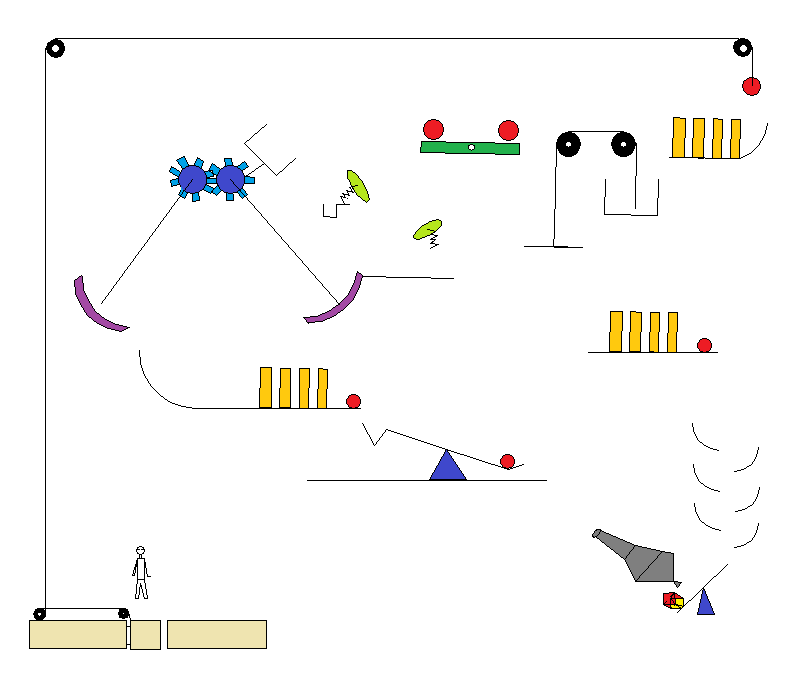
\includegraphics[height=13cm, scale=0.5]{img/Proposed.png} 
\end{center}
A person enters the room and a series of simulations start.\\ \\
First the ball in the top right corner hits the dominos which eventually falls into a box.\\ \\
The box is connected to horizontal bar by 2 pulleys.\\ \\
The horizontal bar raises upward and hits the green horizontal rotating platform.\\ \\
The balls on the top of rotating platform fall on the springs and eventually onto the gears.\\\\
The gears rotate and the ball falls on the dominos which eventually disturbs another ball .\\ \\
This disturbed ball falls on the see-saw and the ball on the other side disturbs dominos.\\ \\
Finally the ball on the right of dominos falls and initiates the canon and the bullet is fired.\\\\
He has to solve the puzzle and if he fails to do in the specific time he will be fired.\\ \\
}
\clearpage


\section{\large{PROJECT IMPLEMENTATION}}
\large{
Main parts in the simulation are still used but the design is changed.\\ \\
The theme of security system is maintained. \\
\begin{center}
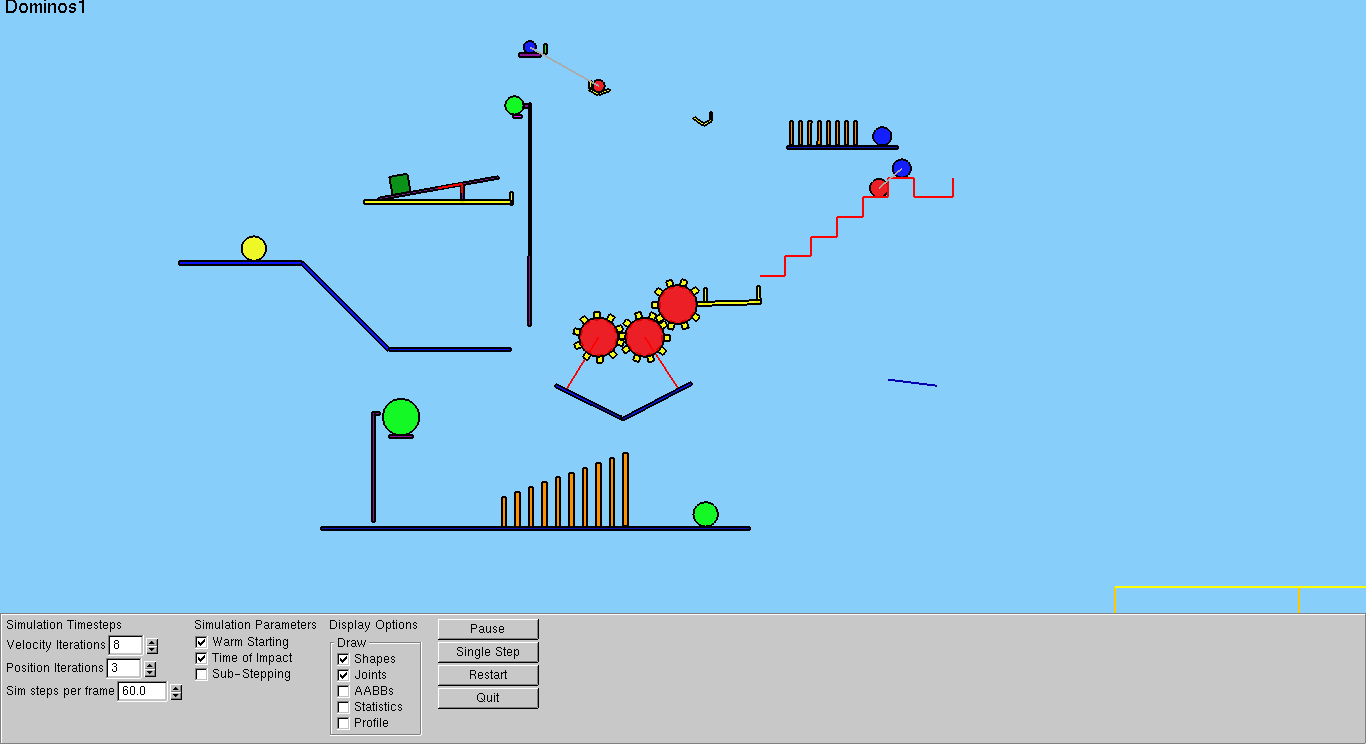
\includegraphics[height=13cm, scale=0.5]{img/middle.png}    %Change to implemented
\end{center}
Here a car enters the room and starts the simulation.\\\\
The car hits the rod and by the Pascal's rule the piston on the other side hits the blue ball.\\\\
The system then travels towards right and hits the yellow ball.\\ \\
Then a series of simulations occur and finally the ball reaches near maze.\\\\\
If the person is unable to solve the puzzle then the car will be blown. \\\\
}
\clearpage


\section{MACHINE INTERNALS}

\subsection*{Gear system}
\begin{center}
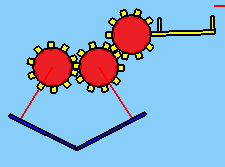
\includegraphics[height=4cm]{img/gears.png}    
\end{center}
When one sphere rotates the others rotate due to the the teeth alignment.\\
\begin{center}
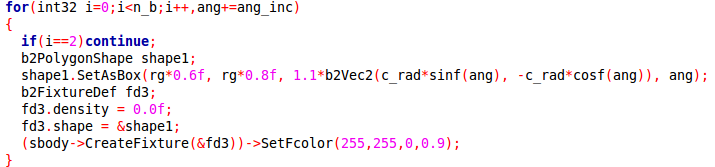
\includegraphics[height=4cm]{img/gearTeeth.png}    
\end{center}

\subsection*{RopeJoint}
\begin{center}
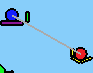
\includegraphics[height=4cm]{img/ropeJoint.png}    
\end{center}
\begin{center}
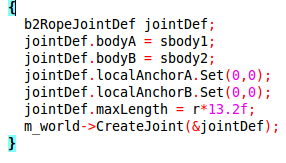
\includegraphics[height=4cm]{img/ropeJointImplementation.png}    
\end{center}

\subsection*{Maze}
\begin{center}
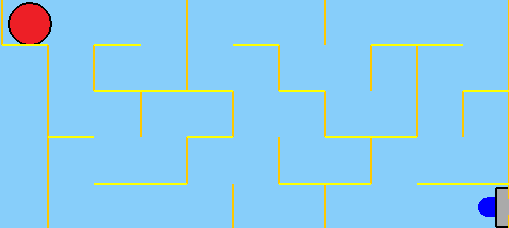
\includegraphics[height=4cm]{img/maze.png}    
\end{center}

\clearpage
\section{\large{WORKING ON THE PROJECT}}

\large{
\vspace{40pt}
\section{\large{DISTRIBUTION OF WORK}}
\large{
Sahil:\\
Most of the project is done by him including adding the colors , propsing the design , modifying most of the code of the individual elements and arranging them.\\
Rajesh:\\
Proposed the idea of the project ,design , wrote code for maze,some other small elements and did the documentation part including srs and slides
ManiTeja:\\
Proposed the design , did the documentation part and implemented some objects.
}
\section{\large{ DIFFICULTIES FACED}}
\large{
We changed a lot from the design we proposed and the one we did.The main reason for that is we figured out that many  elements are repetitive and are not interesting at all.We faced difficulties while designing the simulation and using some classes like Contact listener,Mouse Joint etc.Apart from that everything else is fun and easy.
}
}
\clearpage
\section*{\large{PROJECT SUMMARY}}
\large{
Our cs251 project is a 2D rube Goldberg machine implemented on the Box2D physics simulator.\\
 It is the simulation of a series of processes which results in the event of ”firing a bullet from canon”.\\
It serves the purpose of a security system.\\
 The working of this machine depends on the synchronous working of the following separate components (as given in the figure) .\\

\large{
We did this project as a part of the assignment , But we had a real experience on how a project is done.\\
We learnt  the following as a part of the project: \\
\\
{\huge Non Technical:}\\
\\
1.Team Work\\
2.Better Efficiency in doing large projects\\
3.Project management\\
4.Facing difficulties  and how we had to change our Project Proposal accordingly\\
\\
\\
{\huge Technical:}\\
\\
1.Using Box2d \\
2.Makefiles and all shell commands \\
3.Documentation using Doxygen\\
4.Presentation in Beamer and Bibtex\\
}
}
\clearpage
\section*{}
\hfill
\begin{thebibliography}{7}

\bibitem{einstein} 
\href{''http://box2d.org/''}{Box2D Website}

\bibitem{einstein} 
\href{''https://www.youtube.com/watch?v=0kqIChxrw-4''}{https://www.youtube.com/watch?v=0kqIChxrw4}

\bibitem{einstein} 
\href{''https://www.youtube.com/watch?v=bBIXpu-D_Zo''}{https://www.youtube.com/watch?v=bBIXpuDZo}

\bibitem{einstein} 
\href{''https://www.youtube.com/results?search_query=box2d''}{https://www.youtube.com/results?searchquery=box2d}
 
\bibitem{einstein} 
\href{''https://www.youtube.com/watch?v=8kZRpouZ3OQ''}{https://www.youtube.com/watch?v=8kZRpouZ3OQ}

\bibitem{einstein} 
\href{''https://www.youtube.com/watch?v=9fCT-EjlF9I''}{https://www.youtube.com/watch?v=9fCTEjlF9I}

\end{thebibliography}
\clearpage


\end{document}

